\documentclass[conference,letterpaper]{IEEEtran}
\usepackage[T1]{fontenc}
\usepackage[utf8]{inputenc}
\usepackage{cite,amsmath,amssymb,booktabs,graphicx,array,tabularx,xurl,microtype}
\usepackage{tikz}
\usetikzlibrary{arrows.meta,positioning}
\usepackage[hidelinks,pdfauthor={Jepson Taylor},pdftitle={Prefix-Limited Forecasting of PLGA Drug Release: Kinetic Features and Grouped Evaluation},pdfsubject={Amphora technical white paper draft}]{hyperref}
\urlstyle{same}
\newcolumntype{Y}{>{\raggedright\arraybackslash}X}
\newcommand{\clip}{\operatorname{clip}_{[0,1]}}
\newcommand{\MAE}{\operatorname{MAE}}
\newcommand{\code}[1]{\texttt{#1}}
% Generated from audited aggregate metrics; no raw observations.
\newcommand{\StageRows}{
Raw prefix & 13.798 & 13.592 \\
All candidates & 13.077 & 13.472 \\
Minimum error & 13.535 & 13.169 \\
Pareto selection & 13.348 & 13.139 \\
All + Pareto & 13.104 & 13.544 \\
First-order residual & 13.145 & 13.867 \\
}
\newcommand{\ContrastRows}{
RF & All - Raw & -0.720 & [-1.473, +0.191] & 0.812 \\
RF & Pareto - All & +0.270 & [-0.338, +0.883] & 1.000 \\
RF & Pareto - Minimum & -0.187 & [-0.469, +0.065] & 1.000 \\
RF & All + Pareto - All & +0.027 & [-0.188, +0.220] & 1.000 \\
RF & Residual - All + Pareto & +0.041 & [-0.524, +0.506] & 1.000 \\
LGBM & All - Raw & -0.120 & [-0.935, +0.903] & 1.000 \\
LGBM & Pareto - All & -0.334 & [-1.078, +0.246] & 1.000 \\
LGBM & Pareto - Minimum & -0.030 & [-0.395, +0.280] & 1.000 \\
LGBM & All + Pareto - All & +0.072 & [-0.594, +0.574] & 1.000 \\
LGBM & Residual - All + Pareto & +0.323 & [-0.460, +0.846] & 1.000 \\
}
\newcommand{\PilotRows}{
Persistence & 40.730 & 40.730 \\
Linear & 23.204 & 23.204 \\
Higuchi & 23.946 & 23.946 \\
First order & 19.324 & 19.324 \\
Standalone Pareto & 26.840 & 26.840 \\
Random Forest & 14.375 & 14.176 \\
Histogram boosting & 13.959 & 13.726 \\
RF + Pareto & 13.470 & 13.633 \\
}

\title{Prefix-Limited Forecasting of PLGA Drug Release:\\Kinetic Features and Grouped Evaluation}
\author{\IEEEauthorblockN{Jepson Taylor}\IEEEauthorblockA{Amphora technical white paper draft\\18 October 2026}}
\pagestyle{plain}
\begin{document}
\maketitle
\begin{abstract}
Forecasting the unobserved portion of a drug-release curve requires a precise statement of what is visible when a prediction is made. This paper presents an Amphora benchmark that restricts every target formulation to its first three valid recorded observations and evaluates predictions only at subsequent observed times. An audited transformation of the Bao PLGA corpus retains 320 formulations and 3,910 suffix targets. The third observation occurs at a median of 1.93 days; the prefix is not a fixed 24-hour assay budget. An exploratory pilot is followed by a frozen, post-pilot internal evaluation using 78 connected drug/publication blocks, nested model selection, two tree learners, and six matched representation arms. Random Forest with ordinary kinetic summaries obtains 13.077 percentage points of formulation-balanced suffix mean absolute error, compared with 13.798 for raw-prefix inputs; LightGBM with Pareto selection obtains 13.139 compared with 13.592. All ten planned conditional 95\% intervals include zero, and no contrast survives Holm correction. The contribution is an explicit information boundary, controlled characterization of kinetic representations, and a low-compute, replayable evidence workflow rather than an established Pareto-specific accuracy gain. All 1,560 fits, including full fresh-process replay, completed with byte-identical predictions, search scores, and selected configurations. External prospective validation remains the next scientific step.
\end{abstract}
\begin{IEEEkeywords}
drug release, PLGA, prefix forecasting, kinetic features, grouped cross-validation, reproducibility
\end{IEEEkeywords}

\section{Introduction}
Poly(lactic-co-glycolic acid) (PLGA) formulations offer a useful setting for data-driven release forecasting because formulation properties, manufacturing choices, and the observed time course jointly determine the prediction problem. Existing work has demonstrated that machine learning can inform the design of polymeric long-acting injectables \cite{bannigan2023}. The engineering question considered here is narrower: after a short recorded prefix of a formulation's in-vitro curve is available, how should its later cumulative release be estimated, and what evidence distinguishes useful kinetic information from the selection rule used to summarize it?

A retrospective dataset contains information that would not yet be available during an early formulation decision. Whole-curve kinetic fits, terminal release, and normalization by final duration can change the information content of a benchmark even when a train/test split is otherwise valid. A forecast must therefore specify both the population separation and the within-formulation information boundary. We expose three recorded time/release pairs, formulation metadata, and a requested future time. Future release values enter scoring only. The requested times are the observed suffix times in the retained archive; they are not a prospectively designed sampling schedule.

The present study provides three concrete contributions. First, it instantiates a fully specified first-three-record task with retained cleaning rules, units, group assignments, and immutable code/protocol identifiers. Second, it compares raw-prefix, ordinary kinetic, minimum-error, and Pareto representations under matched learner budgets, including a direct-versus-residual control. Third, it retains full prediction and model-selection evidence and verifies exact fresh-process replay within a bounded CPU environment. These contributions support scrutiny and reuse even when an accuracy advantage is uncertain.

Amphora supplies the research codebase and an existing mathematical Pareto-ranking primitive. The executed benchmark is an isolated adapter around that primitive, not a qualification of a complete autonomous research engine or a pretrained biological model. No large-language-model calls, molecular simulation, laboratory experiments, or production services are part of the reported computation. The public merged source contains the two benchmark modules and their provenance \cite{amphora2026}; the manuscript uses their audited outputs without new model fitting.

The empirical result is deliberately specific. Ordinary kinetic summaries and Pareto summaries can both yield favorable point estimates relative to a raw-prefix learner. However, adding Pareto summaries to ordinary kinetic information does not improve either learner's point estimate in the post-pilot campaign, and every planned interval spans zero. The evidence characterizes the representations and their uncertainty; it does not establish predictive supremacy or statistical equivalence.

\section{Related Work and Positioning}
Bannigan \emph{et al.} already included release measurements at 6, 12, and 24 hours and used nested cross-validation \cite{bannigan2023}. Their grouping by drug--polymer combination differs from a jointly drug-identity-and-publication-disjoint partition, and their discussion acknowledges individual-drug overlap between sets. Thus, neither early-release inputs nor nested selection is introduced here as a new concept.

Alabsi \emph{et al.} predict release beyond 24 hours using formulation descriptors and early release information from a harmonized collection of 347 formulations and 5,265 measurements \cite{alabsi2026}. They examine information ablations, kinetic parameters, and ensemble trees, with formulation-grouped evaluation. The present ordinary-kinetic comparator is motivated by this literature and by its public model card \cite{alabsiModelCard}. It is reimplemented with an explicit prefix-only fitting boundary; it is not an exact reproduction of their pipeline. We do not infer an information-boundary violation from differences in the reported setup.

MC-NODE decomposes release dynamics into structured components and a neural residual, and evaluates DOI-grouped, drug-grouped, and fingerprint-cluster settings \cite{tang2026}. Its sparse-time analysis reduces observations in training curves while evaluating complete test curves; the original sparse rule retains both endpoints. Conditioning a target curve on its first three recorded observations is a different information setting. Its whole-trajectory RMSE cannot be compared numerically with the suffix MAE reported here. Drug identity separation also does not imply fingerprint-cluster separation.

Table~\ref{tab:positioning} summarizes the distinctions relevant to this paper. Group-aware validation and nested model selection are established methodology \cite{roberts2017,varma2006}. The contribution is the auditable combination of a recorded-prefix boundary, connected drug/DOI blocks, and a matched representation experiment, rather than a priority claim about generic early-release prediction, hybrid kinetics, residual learning, or grouped benchmarking.

\begin{table*}[t]
\caption{Related evaluation settings. Different target definitions and information boundaries preclude direct cross-paper score rankings.}
\label{tab:positioning}
\centering\small
\begin{tabularx}{\textwidth}{@{}p{.16\textwidth}YYY@{}}\toprule
Study & Temporal information / task & Grouping relevant to comparison & Relationship to this study \\\midrule
Bannigan \emph{et al.} \cite{bannigan2023} & Includes 6/12/24-hour release inputs & Nested evaluation with drug--polymer combinations & Establishes prior early-input and nested-model-selection work \\
Alabsi \emph{et al.} \cite{alabsi2026} & Early information and kinetic features; targets beyond one day & Formulation-grouped evaluation & Motivates ordinary kinetic/tree controls; not reproduced exactly \\
MC-NODE \cite{tang2026} & Continuous trajectories; sparse training-time supervision & DOI, drug, and chemical-cluster protocols & Prior mechanistic/residual and grouped evaluation; a different target-prefix task \\
This work & First three valid distinct-time records; later observed targets & Joint connected drug/DOI blocks; nested stage-2 selection & Matched all/minimum/Pareto summaries and direct/residual controls \\\bottomrule
\end{tabularx}
\end{table*}

\section{Data and Forecasting Task}
\subsection{Source, Units, and Cohort Construction}
The sole source corpus is the Bao collection \cite{bao2025,baoData2024}. We use version-2 Mendeley metadata and its official formulation table, together with two processed tables pinned to a public derivative repository revision. The derivative contains 321 formulation rows and 4,913 release observations. IDs join one-to-one to the official table; drug SMILES agree exactly and loading values agree numerically. All source formulations have publication DOI metadata. The retained cohort represents 113 publication DOIs. The separate 181-formulation archive associated with earlier work is not unioned into this benchmark.

Time is expressed in days and cumulative release as a fraction. Before scoring, the pilot fixes a validity rule requiring finite nonnegative time and finite release in $[-0.02,1.02]$. Thirty-five supra-range release rows are excluded; four duplicate-time rows are collapsed by averaging release at identical formulation/time coordinates. These are retained inclusion rules, not a finding that the original observations are erroneous. Formulation 74 has six original records but only four valid distinct times after cleaning and fails the minimum of five. The eligible cohort therefore contains 320 formulations, 4,870 valid distinct-time observations, and 3,910 suffix targets. The minimum length supplies at least two scored suffix observations after the three-record prefix.

There is no interpolation, final-release normalization, or scaling by whole-curve duration. The first three observations are selected after the frozen cleaning and duplicate-time rules. Eligibility is retrospective: the archive must contain a sufficiently long valid curve to score a suffix. This selection should not be interpreted as the population encountered in a prospective early-screening experiment.

\subsection{Visible Information and the Estimand}
For formulation $i$, let ordered valid observations be
$\{(t_{ij},y_{ij})\}_{j=1}^{m_i}$, where $m_i\geq5$.
The visible prefix and scored suffix are
\begin{align}
 P_i&=\{(t_{ij},y_{ij}):j\leq3\},\\
 Q_i&=\{t_{ij}:j>3\}.
\end{align}
At a requested $t\in Q_i$, prediction is $\hat y_i(t)=f(x_i,P_i,t)$, with $x_i$ containing formulation metadata. No $y_{ij}$ for $j>3$ is a predictor argument. Ten numeric descriptors cover drug physicochemical properties, polymer/particle properties, loading, encapsulation, and enhancer concentration; formulation method is categorical. Formulation ID and SMILES are excluded as prediction features. SMILES and descriptors are used separately to construct grouping identities.

The primary metric is formulation-balanced suffix MAE in percentage points (pp):
\begin{equation}\label{eq:mae}
 M=\frac{100}{N}\sum_{i=1}^{N}\frac{1}{m_i-3}
       \sum_{j=4}^{m_i}|y_{ij}-\hat y_i(t_{ij})|.
\end{equation}
Thus, a curve with many digitized points does not dominate the headline metric. This differs from pooled row-weighted MAE, whole-curve RMSE, or a time-integrated trajectory error. Repeated pilot predictions are averaged at the per-formulation loss level before uncertainty calculations.

\subsection{What Three Records Mean}
In 317 of 320 formulations the prefix includes the record $(0,0)$. The budget is therefore usually two positive-time observations plus a recorded origin, not three new independent assays. The third time has median 1.928 days, interquartile range 0.744--2.945 days, and range 0.0217--21.072 days. Prefixes end by day 1 in 111 formulations and by day 3 in 248. Figure~\ref{fig:timing} shows this heterogeneity. A first-three-record task is not equivalent to a fixed 24-hour window, and its retrospective error does not establish a time-saving claim for an assay program.

\begin{figure}[t]
\centering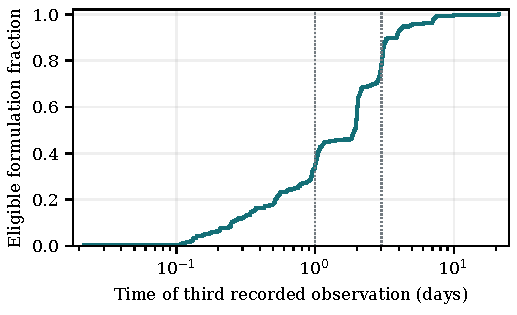
\includegraphics[width=\columnwidth]{figures/prefix_timing.pdf}
\caption{Empirical distribution of the third valid recorded time over the 320 eligible formulations. Dotted guides mark one and three days. The prefix budget is record-based, with nonuniform elapsed time; the plotted distribution is derived from the retained cohort, not a new experiment.}
\label{fig:timing}
\end{figure}

\section{Prefix-Only Representations}
\subsection{Shared Kinetic Candidate Pool}
The pilot uses persistence, linear, Higuchi, and first-order forecasts. Persistence returns the last visible release. Linear and Higuchi fits use a nonnegative coefficient on $t-t_1$ or $\sqrt t-\sqrt{t_1}$, anchored at the clipped first release and bounded below by the last visible release. A transformed least-squares first-order fit uses the remaining fraction, producing a forecast of the form
\begin{equation}
 z_{\mathrm{FO}}(t)=1-(1-a_0)\exp[-k\max(0,t-t_1)],
\end{equation}
where $a_0=\clip(y_1)$ and $k\geq0$; the last-visible-release lower bound and $[0,1]$ clipping are applied. These operations follow the archived implementation exactly.

Stage 2 adds bounded Korsmeyer--Peppas (KP) \cite{korsmeyer1983} and Weibull \cite{langenburg1972} families:
\begin{align}
 z_{\mathrm{KP}}(t)&=k_{\mathrm{KP}}t^n,\\
 z_{\mathrm{W}}(t)&=1-\exp[-(t/\alpha)^\beta].
\end{align}
KP uses a log-linear fit on positive time/release records, with $n\in[0.1,2]$ and $k_{\mathrm{KP}}\in[10^{-6},10]$. Weibull uses the log--log transform for $t>0$ and $0<y<1$, with $\beta\in[0.1,3]$ and $\alpha\in[10^{-3},10^4]$ days. The intercept is recomputed after exponent clipping. At least two usable distinct transformed times are required; otherwise the prefix-only first-order forecast is substituted. All candidate forecasts are clipped to $[0,1]$.

These are small phenomenological feature models. In 317 profiles both two-parameter families have exactly two usable positive-time points when fitted to the full prefix, leaving no residual degrees of freedom for assessing their physical adequacy. Parameter bounds, fit counts, fallback flags, and descriptive prefix $R^2$ values are retained. The $R^2$ values do not identify a release mechanism, and a KP exponent is not given a causal interpretation in this experiment.

\subsection{Selection and Refitting}
For every candidate $c$, a prefix-validation error is obtained by fitting the first two records and predicting the third:
\begin{equation}
 e_{ic}=|y_{i3}-z_c(t_{i3};P_i^{(2)})|.
\end{equation}
The candidates are then refitted using all three visible records for suffix prediction. In the common zero-origin setting, KP and Weibull may fall back to first order during the two-record selection fit, even though their full-prefix fit is available. Complexity is a fixed nominal family count, including under fallback: $(0,1,1,1,2,2)$ in the stage-2 pool order persistence, linear, Higuchi, first order, KP, and Weibull.

The existing Amphora primitive ranks $(e_{ic},d_c)$ by Pareto dominance, minimizing both prefix error and nominal complexity. The non-dominated front is retained; its query-time mean, standard deviation, and size are the three Pareto summary features. The pilot applies the same rule to its four-family pool with complexities $(0,1,1,1)$. This is a finite candidate ranking operation, not a full evolutionary search.

The ordinary control averages every admissible candidate forecast and retains its standard deviation and pool size. The minimum-error control selects the smallest $e_{ic}$, breaking ties in fixed candidate order; its three columns are the chosen forecast, zero standard deviation, and count one. All three controls share the same candidate fits and prediction budget. Their added column count is matched, although constant columns mean their effective feature complexity need not be identical.

\subsection{Six Stage-2 Arms}
Raw inputs comprise static descriptors, method, the three times and releases, prefix mean/last value/slope/duration, and query time, $\log(1+t)$, and elapsed time from the prefix end. Table~\ref{tab:arms} defines every representation. The common kinetic block has ten columns: the two KP and two Weibull parameters, two prefix $R^2$ values, two usable-point counts, and two fallback flags.

\begin{table}[t]
\caption{All frozen stage-2 arms. Each is evaluated with both learners.}
\label{tab:arms}\centering\small
\begin{tabularx}{\columnwidth}{@{}lY@{}}\toprule
Arm & Features added to raw inputs / target \\\midrule
Raw & None; direct release target \\
All & Common kinetic block + all-candidate mean/std/count \\
Minimum & Common block + minimum-error forecast/0/1 \\
Pareto & Common block + front mean/std/count \\
Combined & Common block + all-candidate and Pareto summaries \\
Residual & Exactly the combined features; first-order residual target \\\bottomrule
\end{tabularx}
\end{table}

The residual arm fits $r_i(t)=y_i(t)-z_{\mathrm{FO},i}(t)$ using the same features, learner, splits, and grid as the direct combined arm. It returns
\begin{equation}
 \hat y_i(t)=\clip\{z_{\mathrm{FO},i}(t)+\hat r_i(t)\}.
\end{equation}
The anchor uses only the visible prefix. This is an attribution control for the target parameterization, not a claim to introduce kinetic-residual prediction. Pointwise clipping bounds outputs but does not impose a monotone learned trajectory.

\begin{figure*}[t]
\centering
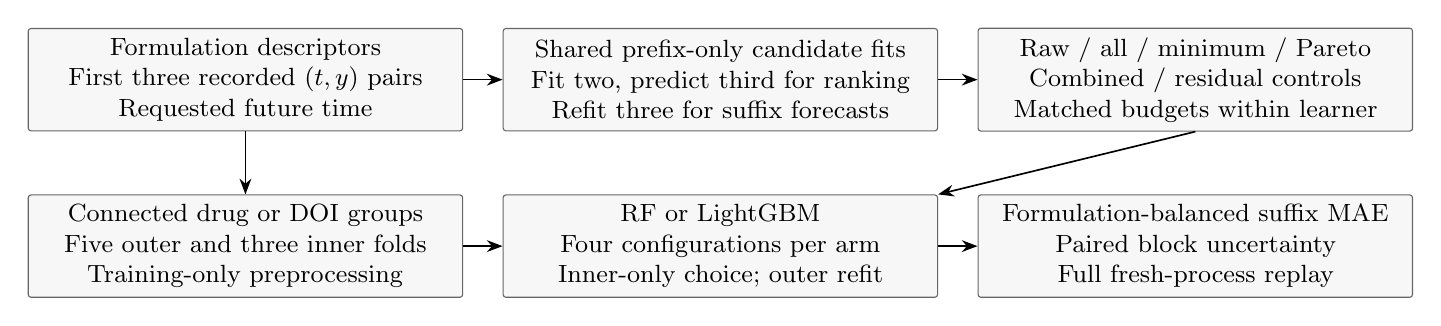
\begin{tikzpicture}[node distance=5mm and 5mm,box/.style={draw=black!60,rounded corners=1pt,fill=black!3,text width=2.08in,minimum height=13mm,align=center,font=\small},arr/.style={-{Stealth[length=2mm]},line width=.6pt}]
\node[box] (input) {Formulation descriptors\\First three recorded $(t,y)$ pairs\\Requested future time};
\node[box,right=of input] (pool) {Shared prefix-only candidate fits\\Fit two, predict third for ranking\\Refit three for suffix forecasts};
\node[box,right=of pool] (arms) {Raw / all / minimum / Pareto\\Combined / residual controls\\Matched budgets within learner};
\node[box,below=8mm of input] (groups) {Connected drug or DOI groups\\Five outer and three inner folds\\Training-only preprocessing};
\node[box,right=of groups] (learn) {RF or LightGBM\\Four configurations per arm\\Inner-only choice; outer refit};
\node[box,right=of learn] (score) {Formulation-balanced suffix MAE\\Paired block uncertainty\\Full fresh-process replay};
\draw[arr] (input)--(pool);\draw[arr] (pool)--(arms);\draw[arr] (groups)--(learn);\draw[arr] (learn)--(score);\draw[arr] (arms.south)--(learn.north east);\draw[arr] (input)--(groups);
\end{tikzpicture}
\caption{Executed information and evaluation boundaries. The shared candidate calculations see a target formulation's prefix only. Global learners and preprocessing fit training formulations only; held-out future releases are used exclusively to score the resulting predictions. The diagram describes the benchmark adapter and does not imply execution by a full autonomous campaign engine.}
\label{fig:boundary}
\end{figure*}

\section{Evaluation Design}
\subsection{Drug and Publication Components}
The pilot's primary groups connect exact drug SMILES or equality of drug molecular weight, topological polar surface area, and logP rounded to six decimals. The eligible data form 88 drug components. The joint sensitivity connects a shared drug component \emph{or} a normalized official DOI, producing 78 connected components; the largest contains 59 formulations. The same joint grouping is used in stage 2. Connected components prevent a chain of linked drugs and publications from crossing a partition. They do not guarantee separation by chemical scaffold, fingerprint cluster, laboratory, or all possible unpublished dependencies.

Independent reconstruction verifies component membership and every retained partition. No drug group or DOI crosses a joint training/held-out boundary. Publication overlap remains in 14 of 15 primary drug-only pilot folds; hence the pilot primary result alone is not publication-independent. Stage-2 held-out fold sizes are 43, 83, 93, 48, and 53 formulations. Unequal component sizes explain this imbalance; no row-level random split is used.

\subsection{Exploratory Pilot and Post-Pilot Campaign}
The primary pilot uses three shuffled five-fold group partitions with seeds 20261017--20261019, fixed models, and no hyperparameter search. Each formulation is held out once per repeat, yielding 960 curve evaluations per analysis, not 960 independent formulations. Eight models include the four kinetic families, standalone Pareto, RF, histogram gradient boosting, and RF augmented with three Pareto features. RF uses 128 trees and leaf minimum three; boosting uses 128 iterations, 15 leaves, learning rate 0.05, and $L_2$ regularization one.

The original RF thread count was changed from two to one after an unscored floating-point replay failure and before the first valid score. The retained amended primary lock precedes scoring. Joint drug/DOI blocking was selected after primary results and locked before its own scores. Boosting paired intervals were added during the later audit. These chronological distinctions are part of the evidence record; the sensitivity does not replace the original primary analysis.

Stage 2 is explicitly \emph{post-pilot internal validation}. Every Bao curve had already been examined. The complete arm list, grids, contrast family, seeds, and stopping rule were frozen before stage-2 scoring, but that freeze does not erase prior corpus exposure. New outer folds therefore protect the within-run selection boundary without becoming an untouched external test. No model family, feature arm, or seed was subsequently adapted to outer scores.

Stage 2 shuffles sorted joint-component IDs with seed 20261020 and assigns them round-robin to five outer folds. Within each outer training set, the same procedure creates three inner folds with seed $20261100+k$, where $k\in\{0,\ldots,4\}$ is the outer index. Median imputation and one-hot method encoding are fitted separately to each inner training split and outer refit. Unknown categories are ignored. A formulation's training rows have equal total weight, rescaled so mean row weight is one. Configuration choice minimizes pooled inner out-of-fold formulation MAE, with fixed grid index as a tie-break; outer labels do not choose configurations or a winning learner family.

\subsection{Matched Search Budgets}
RF \cite{breiman2001} has 128 trees, one thread, and four configurations from minimum leaf size $\{2,6\}$ crossed with maximum feature fraction $\{0.7,1.0\}$. LightGBM \cite{ke2017} has 256 estimators, learning rate 0.05, $L_2$ regularization one, and four configurations from leaf count $\{7,15\}$ crossed with minimum child samples $\{10,25\}$. Deterministic column-wise LightGBM fitting and fixed seed 20261020 are used. There is no early stopping or adaptive expansion of either grid. These are bounded matched searches, not an exhaustive claim about the best possible tree model.

For six arms, two learners, and five outer folds, the fit budget is
\begin{equation}
 6\times2\times5\times(4\times3+1)=780.
\end{equation}
A fresh-process repetition of the full matrix gives 1,560 fits in total. Replay doubles computational work, not the number of independent scientific evaluations.

\subsection{Conditional Uncertainty and Multiplicity}
The pilot uses 2,000 paired resamples of drug or joint components after each formulation's losses are averaged over repeats. Stage 2 uses 5,000 paired resamples of its 78 joint components. Each draw includes all formulations from a selected block and computes the ratio of summed formulation losses to the summed number of formulations; the estimand remains Eq.~\eqref{eq:mae}, not an equal-weight mean of block means.

For each learner, the frozen contrasts are all minus raw, Pareto minus all, Pareto minus minimum, combined minus all, and residual minus direct combined. If $\hat\Delta$ is a loss difference and $\Delta_b^*$ its bootstrap draw, the reported descriptive centered-bootstrap two-sided value is
\begin{equation}
 p=\frac{1+\sum_{b=1}^{B}\mathbf{1}\{ |\Delta_b^*-\hat\Delta|\geq|\hat\Delta|\}}{B+1}.
\end{equation}
Percentile 2.5/97.5\% limits accompany the point differences. Holm correction is applied across all ten contrasts \cite{holm1979}. The retained fits, hyperparameter choices, corpus, and partitions remain fixed during resampling. The intervals do not include campaign-design uncertainty after prior data exposure, retraining variability under resampled datasets, or prospective population shift. Component resampling also relies on the available identity/DOI dependencies adequately capturing the dependence relevant to this conditional summary.

\section{Results}
\subsection{Pilot Context}
Table~\ref{tab:pilot} reports every fixed pilot model. The primary RF augmentation difference is $-0.905$ pp, with a conditional drug-block interval $[-1.459,-0.265]$. With joint blocking, it is $-0.543$ pp with interval $[-1.099,+0.071]$. Augmented RF versus fixed histogram boosting gives $-0.489$ pp $[-1.113,+0.269]$ in the primary analysis and $-0.093$ pp $[-0.643,+0.503]$ in the joint sensitivity; these boosting contrasts are post-results audit comparisons. Standalone Pareto is less accurate than first-order kinetics in this task. The result supports inspecting learned kinetic augmentation, not treating the ranking primitive itself as a sufficient forecasting model.

\begin{table}[t]
\caption{Exploratory pilot MAE (pp). Both analyses use the same cohort and suffix definition; the joint analysis is a later grouping sensitivity.}
\label{tab:pilot}\centering\small
\begin{tabular}{@{}lrr@{}}\toprule
Model & Drug primary & Joint drug/DOI \\\midrule
\PilotRows
\bottomrule\end{tabular}
\end{table}

\subsection{Complete Stage-2 Matrix}
Table~\ref{tab:stage2} retains all twelve learner/arm combinations. RF ordinary kinetics has a point estimate of 13.077 pp versus 13.798 for raw inputs, a difference of $-0.720$ pp with interval $[-1.473,+0.191]$. LightGBM Pareto has 13.139 pp versus 13.592 for raw inputs; the latter juxtaposition is descriptive, while the planned attribution contrasts are retained as a fixed family. Neither selecting a favorable row nor comparing stage-2 values with the differently configured pilot provides a confirmatory test.

\begin{table}[t]
\caption{Complete stage-2 formulation-balanced suffix MAE (pp). Lower is better. The arms are defined in Table~\ref{tab:arms}; no row is selected as a confirmed winner.}
\label{tab:stage2}\centering\small
\begin{tabular}{@{}lrr@{}}\toprule
Representation / target & RF & LightGBM \\\midrule
\StageRows
\bottomrule\end{tabular}
\end{table}

The controls change the interpretation of augmentation. RF Pareto minus ordinary all-candidate summaries is $+0.270$ pp $[-0.338,+0.883]$, whereas LightGBM gives $-0.334$ pp $[-1.078,+0.246]$. Relative to minimum-error selection, Pareto differences are $-0.187$ pp $[-0.469,+0.065]$ for RF and $-0.030$ pp $[-0.395,+0.280]$ for LightGBM. Incrementally adding Pareto to ordinary features changes RF by $+0.027$ pp $[-0.188,+0.220]$ and LightGBM by $+0.072$ pp $[-0.594,+0.574]$. The ordinary kinetic information is therefore a necessary comparator when interpreting the earlier RF augmentation estimate.

The residual target also does not improve the direct combined arm's point estimate: RF changes by $+0.041$ pp $[-0.524,+0.506]$, and LightGBM by $+0.323$ pp $[-0.460,+0.846]$. Figure~\ref{fig:contrasts} shows all ten planned intervals. Every interval includes zero. The smallest Holm-adjusted value is 0.812; the other nine are 1.000. This is a lack of resolved comparative evidence under the retained design, not evidence that the representations are equivalent.

\begin{figure*}[t]
\centering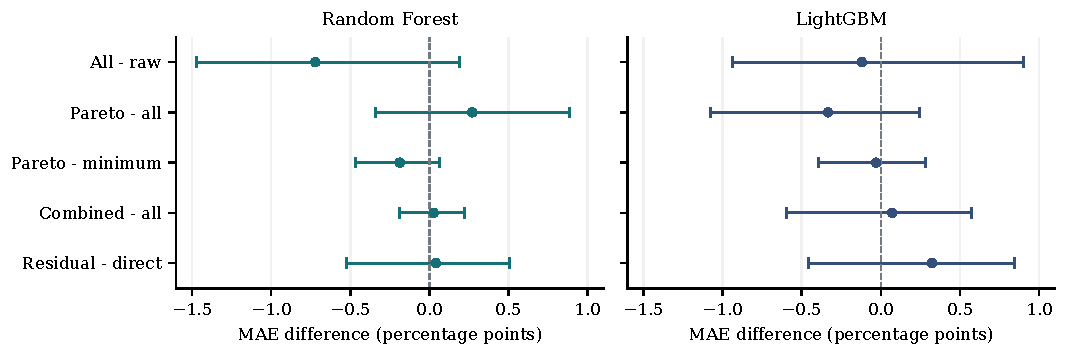
\includegraphics[width=\textwidth]{figures/contrasts.pdf}
\caption{All ten frozen stage-2 contrasts, with paired joint-component percentile 95\% intervals. Negative differences favor the first named representation. ``Combined'' is ordinary plus Pareto summaries; ``direct'' is the corresponding direct-target arm. The intervals are conditional on the exposed corpus and retained fitted procedure. All include zero; no contrast survives Holm correction.}
\label{fig:contrasts}
\end{figure*}

\subsection{Descriptive Recorded-Trajectory Examples}
Figure~\ref{fig:examples} illustrates how the visible prefix and later query points appear in actual out-of-fold predictions. The displayed formulations are the smallest numeric IDs within each tertile of third-observation time. This post-results visualization rule uses prefix timing, not prediction errors or favorable model rankings. Lines connect predictions at recorded target times for readability; they do not indicate interpolated training labels or dense prospective sampling. The examples are descriptive and cannot establish comparative accuracy or physical mechanism.

\begin{figure*}[t]
\centering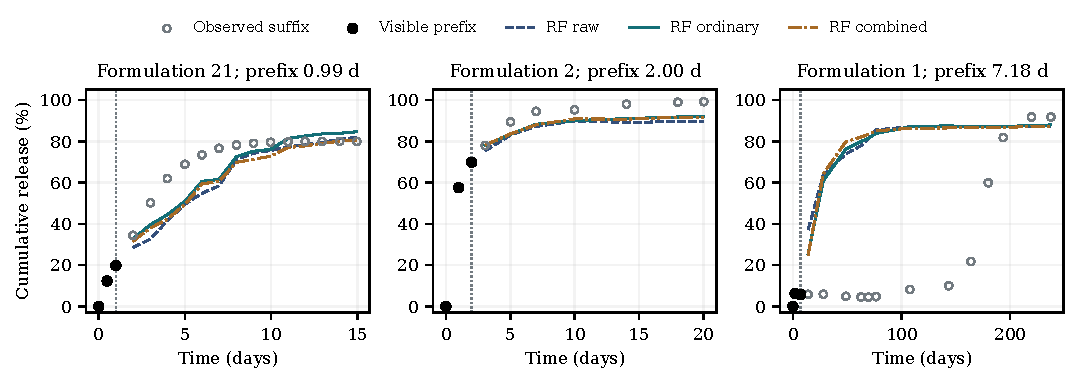
\includegraphics[width=\textwidth]{figures/release_examples.pdf}
\caption{Recorded stage-2 RF predictions for three timing-selected formulations. Black points are the visible prefix; open points are the observed suffix. Vertical dotted guides mark the prefix end. Curves show raw, ordinary kinetic, and combined features from the held-out predictions. Selection is independent of prediction error. Data-derived visualization from Bao version 2 \cite{baoData2024}, with CC BY 4.0 attribution; these are in-vitro archive records, not new laboratory results.}
\label{fig:examples}
\end{figure*}

\section{Reproducibility and Computational Footprint}
The archived workflow records raw-file hashes, official-table joins, cleaning receipts, split assignments, code/protocol digests, every suffix prediction, every inner search score, and selected configurations. Its independent audit recomputes cohort membership, connected components, partition disjointness, the formulation-balanced metric, the planned contrasts, and Holm correction without importing the model-fitting pipeline. A separate fresh-process feature replay perturbs only future release labels and requires byte-identical feature, anchor, and selector receipts for all 320 eligible formulations. Visible-prefix perturbations provide positive controls. These checks establish the implemented information boundary under the tested harness, not the adequacy of the biological data.

For stage 2, all prediction files, inner-search files, and selected-configuration files match byte-for-byte across complete fresh-process runs for both learners: six matching files. The pilot's two full analyses likewise replayed their predictions, metrics, summaries, receipts, and checks, with 1,920 fresh held-out-curve invariance checks passing. Reproduction is established in the recorded environment; no claim is made that arbitrary operating systems or library revisions yield identical floating-point bytes.

Stage-2 main-run process elapsed times are 648.9 s for RF and 54.4 s for LightGBM; replay times are 664.1 s and 54.8 s, respectively. The maximum recorded process resident set is 239.4 MiB. At most two low-priority, single-thread learner processes run concurrently, pinned to two logical CPUs, with a 4-GiB address-space cap per process. Process elapsed times are not summed as a parallel wall-clock measurement. The implementation uses Python 3.12.3, NumPy 1.26.4, pandas 2.3.2, scikit-learn 1.7.2, and LightGBM 4.6.0. No GPU, paid service, or new laboratory measurement is required for the reported analysis.

The computational result is that meaningful representation and evaluation controls are inexpensive enough to retain as part of a small-data release-forecasting workflow. It is not a quantified saving in drug-development cost or assay duration. A desktop disconnect during replay did not interrupt the remote workers; saved outputs were retained, and only summary/audit postprocessing was resumed. No model fits were restarted or selected in response to that interruption.

\section{Interpretation and Next Validation Steps}
The benchmark supplies a useful basis for controlled method development. Its inputs are explicit, candidate fits are small enough to inspect, model-selection budgets are comparable, and the full residual evidence can be replayed. The stage-2 matrix shows why an augmentation estimate should be tested against ordinary kinetic information and a simple selection rule before assigning benefit to Pareto ranking. The method remains a plausible representation option, but its specific advantage is unresolved in this corpus.

Several scientific boundaries shape the next experiment rather than invalidate the computational evidence. The same literature-derived Bao cohort informed the pilot and stage-2 design. DOI/drug grouping is stronger than a random row split for the dependencies it addresses, but does not create chemical-cluster independence or independent assay replicates. Three recorded values often mean only two positive-time points, making two-parameter fits weakly identified. A pointwise tree forecast can be nonmonotone despite bounded outputs. Conditional block intervals leave prospective recruitment, measurement variability, and training-procedure uncertainty unquantified.

A practical next validation should freeze a representation and sampling schedule before examining an overlap-screened new-study PLGA panel. The panel should record assay context, manufacturing provenance, replicate variability, and all candidate outcomes, with a predeclared forecast horizon and comparison margin. A fixed-day schedule would separate the value of early information from the irregular timing of digitized source records. A subsequent ocular application would require its own materials, route, biological context, and external/prospective validation; the present long-acting injectable literature does not establish that transfer. This roadmap extends an auditable workflow while keeping experimental and clinical claims tied to new evidence.

\section{Conclusion}
This work provides an implemented and reproducible combination of prefix-limited forecasting, joint drug/publication separation, and matched kinetic representation controls in the Amphora codebase. The complete recorded evidence is more informative than a selected favorable score: every stage-2 comparison remains uncertain, and no Pareto-specific advantage is established. The positive contribution is a precise, low-compute framework for measuring what a short recorded prefix can support, preserving failed or unfavorable comparisons, and preparing a defensible external validation study. No additional model search is performed for this manuscript.

\appendices
\section{Immutable Reproduction Record}
The public source revision is \href{https://github.com/neverhuman/mvp20-split/tree/879b6d254e10848020635cc2ae2c654968a0cfc1}{\code{879b6d25}}. Original pilot and stage-2 commits are \code{9e4d4afb} and \code{dfac76ae}; their full IDs and links are in the companion README. Full protocol/code SHA-256 values are retained below and in the machine-readable claim ledger. The primary pilot lock is 2026-10-17 22:40:41 UTC, before the first valid score at 22:41:10 UTC; the joint sensitivity lock is 22:44:32 UTC. Stage 2 is locked at 23:12:11 UTC. These are chronological locks, not an independent preregistration.

\begin{table}[h]
\caption{Immutable SHA-256 identifiers (full values).}
\centering\scriptsize
\begin{tabularx}{\columnwidth}{@{}p{.24\columnwidth}X@{}}\toprule
Artifact & SHA-256 \\\midrule
Pilot protocol & \nolinkurl{a3c45e945518cf64c84608df76b5b4c0f551201ef8f24f298692a4e94c1d7a38} \\
Joint protocol & \nolinkurl{71b1b2892c591c085529d5da41b97af208320513b7f25edff47836365ef57034} \\
Stage-2 protocol & \nolinkurl{bc3b78f76a4c24b1643f49384f5546c5f4dd8ee894cf449c33b4f229dc85892d} \\
Pilot pipeline & \nolinkurl{fb963e6001ddfeb8c3cfc7715312dfec5188d982dcbc9f3d84a79f76cf8ba7cc} \\
Stage-2 pipeline & \nolinkurl{712e33f6fd33e9010ce615ef227f24e8af37c6b051e94d86ebc8ce3d6f4fa55a} \\\bottomrule
\end{tabularx}
\end{table}

The processed tables use immutable derivative revision \href{https://github.com/mdsamad001/Drug_Release_Dynamics_Prediction/tree/605cd707c47a4379212193560cd332d7a2d973fd}{\code{605cd707}}; its full identifier and repository URL are retained in the companion README. The official version-2 formulation-table SHA-256 is \nolinkurl{033f01949670afde2aae6d8bdf886b41f6f962170e5d2e5ddf07c520edd51169}. Dataset attribution and CC BY 4.0 terms are retained \cite{baoData2024}; the software retains the repository's existing license/provenance and is not described as newly open-licensed.

The manuscript tree contains source, bibliography, derived figures, and aggregate claim values only. Raw datasets, individual prediction tables, environment directories, and private evidence reports remain outside it. The companion gives verification/build commands and the full ten-contrast table. Building the paper uses the included aggregates and figures; regeneration reads retained evidence and fits no models.

\IEEEtriggeratref{8}
\bibliographystyle{IEEEtran}
\bibliography{references}
\end{document}
